\section{La Tour Phare}

La tour phare de Sichua est visible à des dizaines de kilomètres à la ronde.
Elle est composée de différentes architectures au fur et à mesure des étages.
À son sommet est perché un engin magique emettant une puissante lumière 
utilisée par les marins de haute mer pour se diriger vers le port de Sichua
en toute sécurité. La tour phare est aussi la résidence de l'archimage de la 
ville et de l'école de magie. Ce batiment ancestral est clairement 
d'architecture naine et la demeurre millénaire des plus puissants magiciens 
de la ville.

La tour semble faite d'obsidienne et s'élève a environ 80 mètres sur une 
colline qui en fait autant. Les étages de la base sont principalement 
remplis par la garde et l'école de magie. Le centre de la tour est 
composés des laboratoires et bibliothèques privées des différents 
professeurs et leur assistants. 
Les derniers étages sont réservé à l'archimage et ses assistants personnels.
Une dizaine d'étage pour eux seuls pourrait sembler beaucoup, mais en 
réalité de nombreuses salles sont scellé et en cours d'études. Le mécanisme
d'allumage du phare est entretenu par les assistants de l'archimage et 
occupe les deux derniers etages.

Un secret bien gardé à Sichua est que dans les derniers étages
se trouvent quelques cellules pour les magiciens et autres créatures
qu'il ne serait pas sûr de garder dans la prison principale de Sichua.
L'éspérence de vie de ces personnes est fort limité, lorsqu'elles ont finit
par dire tout ce qu'elle savait ou en tout cas que l'Archimage le pense,
elle servent généralement a des expériences magiques jusqu'à ce que mort
s'en suive...

Les étudiants sont riches -> coût important de l'enseignement

\begin{figure*}[p]
\center
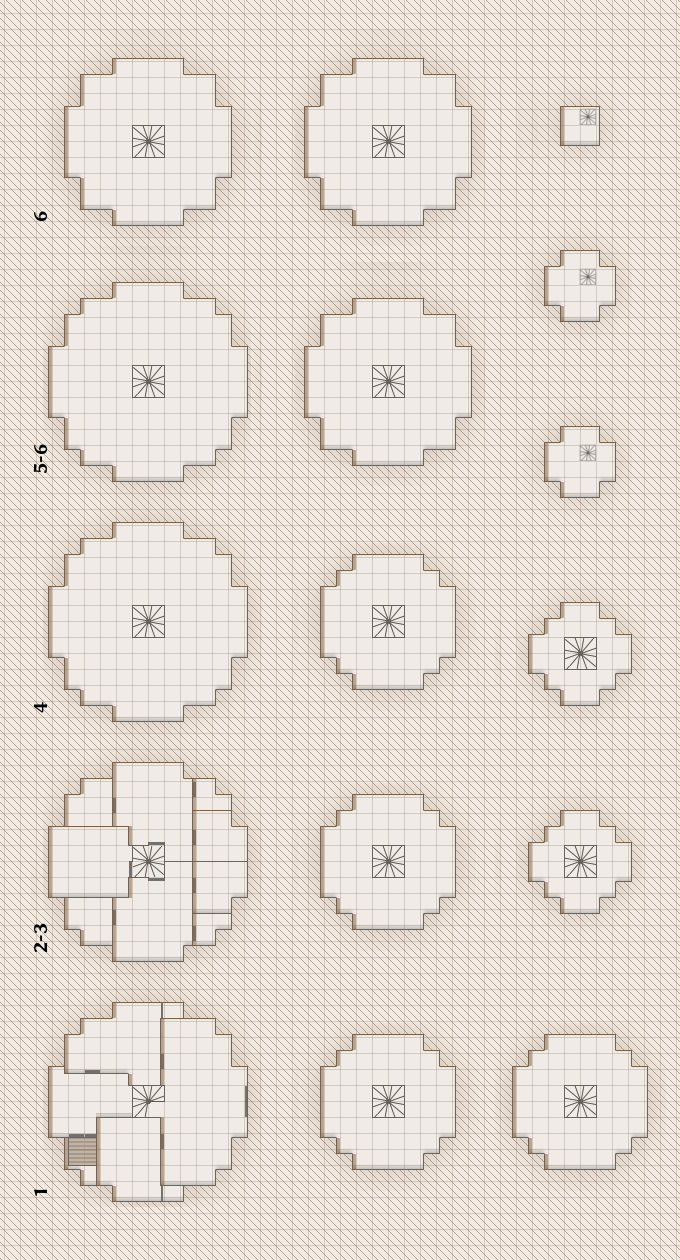
\includegraphics[width=12cm]{Maps/TourMage2.png}
\end{figure*}

